\section{Aufbereitung des Datensatzes}\label{sec:aufbereitung_datensatz}

Bereits beim ersten Schritt einer Machine Learning Pipeline, dem Vorverarbeiten der Daten, können diverse Methoden genutzt werden, um die Vertraulichkeit zu wahren.
In diesem Kapitel werden 3 Kategorien dieser Methoden vorgestellt, und wie diese genutzt werden können, um bereits vor dem eigentlichen Training Modelle sicherer zu machen.

%\subsection{Elimination}
\subsection{Anonymisierung}\label{sec:anonymisierung}

Bei der Anonymisierung von Daten geht es darum, identifizierende Eigenschaften zu entfernen oder unkenntbar zu machen.
Dabei soll dennoch ein gewisser Nutzen erhalten bleiben. 

Sweeney \cite{P-23} stellt eine Methode der Anonymisierung namens \textit{k}-Anonymität (im Englischen \textit{k}-Anonymity) vor.
Die Methode wird im folgenden mittels eines Auszugs des Titanic Datensatzes \cite{D-titanic} erläutert.
Tabelle \ref{tab:nicht_ano_titanic} zeigt einen Auszug aus diesem Datensatz.
Die hier ausgewählten Spalten enthalten beschreibende Merkmale einer Person, sowie Informationen über die Reise auf der Titanic. 
Zur Verdeutlichung gehen wir davon aus, dass es sich bei dem Einstiegsort um eine private Information handelt, die den Wohnort verraten könnte.

\begin{table}[!htb]
\centering
\begin{tabular}{|l|l|l|l|l|}
\hline
\rowcolor[HTML]{EFEFEF} 
Name                     & Geschlecht & Alter & Buchungsklasse & Einstiegsort \\ \hline
Owen Harris Braund       & m          & 22    & 3              & S            \\ \hline
Florence Briggs Thayer   & w          & 38    & 1              & C            \\ \hline
Laina Heikkinen          & w          & 26    & 3              & S            \\ \hline
Lily May Peel            & w          & 35    & 1              & S            \\ \hline
William Henry Allen      & m          & 35    & 3              & S            \\ \hline
Anna McGowan             & w          & 15    & 3              & Q            \\ \hline
James Moran              & m          & 30    & 3              & Q            \\ \hline
Adele Achem Nasser       & w          & 14    & 2              & C            \\ \hline
Don Manuel Uruchurtu     & m          & 40    & 1              & C            \\ \hline
Elizabeth Anne Wilkinson & w          & 29    & 2              & S            \\ \hline
Henry Birkhardt Harris   & m          & 45    & 1              & S            \\ \hline
\end{tabular}
\caption{Nicht-Anonymisierter Titanic Datensatz \cite{D-titanic}}
\label{tab:nicht_ano_titanic}
\end{table}

Bei \textit{k}-Anonymität werden die Attribute in 3 separate Klassen eingeteilt: Identifikatoren, Quasi-Identifikatoren und sensible Attribute.
Bei diesem Beispiel wäre der Name der einzige Identifikator, da über diesen eine Person eindeutig zugeordnet werden kann. 
Quasi-Identifikatoren sind alle Variablen, welche Information über einen Datenpunkt preisgeben, aber nicht direkt auf diesen schließen lassen. 
Um mit Quasi-Identifikatoren einen Datenpunkt zu identifizieren, braucht es in der Regel mehr Informationen, beispielsweise einen Datensatz.
In diesem Beispiel könnte also jede Spalte ein Quasi-Identifikator sein.
Da der Name bereits ein direkter Identifikator ist, wird dieser anders zugeordnet.
Die dritte Klasse sind die sensiblen Attribute, die es zu sichern gilt. 
Hier gehen wir davon aus, dass der Einstiegsort eine schützenswerte Information ist.
Um \textit{k}-Anonymität zu erreichen, muss jede Kombination aus Quasi-Identifikatoren mindestens k mal vorkommen, wobei k festgelegt werden kann. 
Ein größeres k sorgt für mehr Privatsphäre.
Um dies zu erreichen, können die Quasi-Identifikatoren gruppiert werden, so kann beispielsweise anstatt des Alters, eine Zahlenbereich als Alter dienen.
Tabelle \ref{tab:k-ano-titanic} zeigt wie diese Gruppierung aussieht.

% Please add the following required packages to your document preamble:
% \usepackage[table,xcdraw]{xcolor}
% If you use beamer only pass "xcolor=table" option, i.e. \documentclass[xcolor=table]{beamer}
\begin{table}[!htb]
\centering
\begin{tabular}{lllll}
\hline
\rowcolor[HTML]{CBCEFB} 
\multicolumn{1}{|l|}{\cellcolor[HTML]{CBCEFB}Identifikator} & \multicolumn{3}{l|}{\cellcolor[HTML]{CBCEFB}Quasi-Identifikatoren}                                                                                                         & \multicolumn{1}{l|}{\cellcolor[HTML]{CBCEFB}sensibles Attribut} \\ \hline
\rowcolor[HTML]{EFEFEF} 
\multicolumn{1}{|l|}{\cellcolor[HTML]{EFEFEF}Name}          & \multicolumn{1}{l|}{\cellcolor[HTML]{EFEFEF}Geschlecht} & \multicolumn{1}{l|}{\cellcolor[HTML]{EFEFEF}Alter} & \multicolumn{1}{l|}{\cellcolor[HTML]{EFEFEF}Buchungsklasse} & \multicolumn{1}{l|}{\cellcolor[HTML]{EFEFEF}Einstiegsort}       \\ \hline
\multicolumn{1}{|l|}{-}                                     & \multicolumn{1}{l|}{m}                                  & \multicolumn{1}{l|}{20 - 35}                       & \multicolumn{1}{l|}{3}                                      & \multicolumn{1}{l|}{S}                                          \\ \hline
\multicolumn{1}{|l|}{-}                                     & \multicolumn{1}{l|}{m}                                  & \multicolumn{1}{l|}{20 - 35}                       & \multicolumn{1}{l|}{3}                                      & \multicolumn{1}{l|}{S}                                          \\ \hline
\multicolumn{1}{|l|}{-}                                     & \multicolumn{1}{l|}{m}                                  & \multicolumn{1}{l|}{20 - 35}                       & \multicolumn{1}{l|}{3}                                      & \multicolumn{1}{l|}{Q}                                          \\ \hline
                                                            &                                                         &                                                    &                                                             &                                                                 \\ \hline
\multicolumn{1}{|l|}{-}                                     & \multicolumn{1}{l|}{w}                                  & \multicolumn{1}{l|}{15 - 30}                       & \multicolumn{1}{l|}{3}                                      & \multicolumn{1}{l|}{S}                                          \\ \hline
\multicolumn{1}{|l|}{-}                                     & \multicolumn{1}{l|}{w}                                  & \multicolumn{1}{l|}{15 - 30}                       & \multicolumn{1}{l|}{3}                                      & \multicolumn{1}{l|}{Q}                                          \\ \hline
                                                            &                                                         &                                                    &                                                             &                                                                 \\ \hline
\multicolumn{1}{|l|}{-}                                     & \multicolumn{1}{l|}{w}                                  & \multicolumn{1}{l|}{10 - 30}                       & \multicolumn{1}{l|}{2}                                      & \multicolumn{1}{l|}{C}                                          \\ \hline
\multicolumn{1}{|l|}{-}                                     & \multicolumn{1}{l|}{w}                                  & \multicolumn{1}{l|}{10 - 30}                       & \multicolumn{1}{l|}{2}                                      & \multicolumn{1}{l|}{S}                                          \\ \hline
                                                            &                                                         &                                                    &                                                             &                                                                 \\ \hline
\multicolumn{1}{|l|}{-}                                     & \multicolumn{1}{l|}{w}                                  & \multicolumn{1}{l|}{30 - 40}                       & \multicolumn{1}{l|}{1}                                      & \multicolumn{1}{l|}{C}                                          \\ \hline
\multicolumn{1}{|l|}{-}                                     & \multicolumn{1}{l|}{w}                                  & \multicolumn{1}{l|}{30 - 40}                       & \multicolumn{1}{l|}{1}                                      & \multicolumn{1}{l|}{S}                                          \\ \hline
                                                            &                                                         &                                                    &                                                             &                                                                 \\ \hline
\multicolumn{1}{|l|}{-}                                     & \multicolumn{1}{l|}{m}                                  & \multicolumn{1}{l|}{40 - 45}                       & \multicolumn{1}{l|}{1}                                      & \multicolumn{1}{l|}{C}                                          \\ \hline
\multicolumn{1}{|l|}{-}                                     & \multicolumn{1}{l|}{m}                                  & \multicolumn{1}{l|}{40 - 45}                       & \multicolumn{1}{l|}{1}                                      & \multicolumn{1}{l|}{S}                                          \\ \hline
\end{tabular}
\caption{\textbf{k}-Anonymity Titanic Datensat \cite{P-23}\cite{D-titanic}}
\label{tab:k-ano-titanic}
\end{table}

Es ist zu sehen, dass die Identifikatoren, hier nur der Name, entfernt wurden.
Geschlecht und Buchungsklasse sind auch unverändert geblieben.
Die Gruppierung erfolgte anhand der Quasi-Identifikatoren, wobei das Alter durch einen Zahlenbereich ersetzt wurde.
Hier ist anzumerken, dass die Spanne der Altersgruppen unterschiedlich groß ist. 
Je nachdem wie diese Spannen aufgebaut sind, würden sich die Gruppierungen verändern.
\textit{k}-Anonymität mit k = 2 ist hier erfüllt, da jede Kombination von Quasi-Identifikatoren mindestens 2 mal vorkommt.
Dabei ist es auch möglich, dass einzelne Einträge redundant vorkommen. 
So sind in Tabelle \ref{tab:k-ano-titanic} die ersten beiden Einträge identisch, obwohl diese von 2 unterschiedlichen Personen stammen.

Machanavajjhala et al. \cite{P-24} zeigen anhand von 2 Attacken, dass \textit{k}-Anonymität nicht ausreichend ist.
Bei der Homogenitätsattacke kann die Eigenschaft, dass sensible Attribute nicht einzigartig sind, ausgenutzt werden.
Tabelle \ref{tab:homo_k_ano} zeigt abgewandelt die ersten Zeilen der Tabelle \ref{tab:k-ano-titanic}.
Das sensible Attribut, der Einstiegsort, ist jedoch in dieser Quasi-Identifikatoren Kombination identisch.
Sollte also eine Person männlich, zwischen 20 und 35 Jahren alt sein und in der Buchungsklasse 3 mitgefahren sein, so kennt man auch den Einstiegsort.
\begin{table}[!htb]
\centering
\begin{tabular}{|l|lll|l|}
\hline
\rowcolor[HTML]{CBCEFB} 
Identifikator & \multicolumn{3}{l|}{\cellcolor[HTML]{CBCEFB}Quasi-Identifikatoren}                                                            & sensibles Attribut \\ \hline
\rowcolor[HTML]{EFEFEF} 
Name          & \multicolumn{1}{l|}{\cellcolor[HTML]{EFEFEF}Geschlecht} & \multicolumn{1}{l|}{\cellcolor[HTML]{EFEFEF}Alter} & Buchungsklasse & Einstiegsort       \\ \hline
-             & \multicolumn{1}{l|}{m}                                  & \multicolumn{1}{l|}{20 - 35}                       & 3              & S                  \\ \hline
-             & \multicolumn{1}{l|}{m}                                  & \multicolumn{1}{l|}{20 - 35}                       & 3              & S                  \\ \hline
-             & \multicolumn{1}{l|}{m}                                  & \multicolumn{1}{l|}{20 - 35}                       & 3              & S                  \\ \hline
\end{tabular}
\caption{Angreifbare Abwandlung von Tabelle \ref{tab:k-ano-titanic}}
\label{tab:homo_k_ano}
\end{table}

Ein weiteres Problem ist ein Angriff mit Hintergrundwissen, mit dem gewisse sensible Attribute ausgeschlossen werden können oder zumindest unwahrscheinlicher machen könnten.
In diesem Beispiel könnte es also sein, dass ein Angreifer weiß wann, ein Passagier zugestiegen ist und an welchem Hafen das Schiff zu dieser Zeit war. 
Damit können Rückschlüsse auf den Einstiegsort gemacht werden.

Aufgrund dieser beiden Angriffe, schlagen Machanavajjhala et al. \cite{P-24} eine Erweiterung mit dem Namen \textit{l}-Diversität (im Englischen \textit{l}-Diversity) vor.
Dabei wird \textit{k}-Anonymität auf die Daten angewendet und zusätzlich eine Bedingung eingeführt. 
Diese kann sowohl für einen Block, eine einheitliche Kombination der Werte der Quasi-Identifikatoren, als auch für den ganzen Datensatz gelten.
Ein Block ist dabei \textit{l}-divers, wenn die Werte des sensiblen Attributes \textit{\dq gut repräsentiert\dq} sind, wobei l eine Zahl zugeorndet werden kann.
Ist jeder Block des Datensatzes \textit{l}-divers, dann ist auch der ganze Datensatz \textit{l}-divers.
Dabei gibt es 3 Grundvarianten laut Machanavajjhala et al., wie \textit{\dq gut repräsentiert\dq} definiert werden kann \cite{P-24}:
\begin{compactitem}
\item \textbf{Unterscheidbare \textit{l}-Diversität:} Bei dieser Variante, hat ein Block \textit{l} unterschiedliche Werte eines sensiblen Attributes. Ein Block ist daher immer mindestens 1-divers, da dies bedeutet, dass das sensible Attribute immer den gleichen Wert annimmt.
\item \textbf{Entropie \textit{l}-Diversität:} Hier wird die Entropie der sensiblen Attribute eines Blocks berechnet. Dabei ist ein Block \textit{l}-divers, wenn die Entropie $\ge$ log(\textit{l}) ist. Folglich ist 1-Diversität dabei immer gegeben.
\item \textbf{Rekursive (c,\textit{l})-Diversität:} Diese Definition besagt, dass das häufigste sensible Attribut eines Blocks, seltener vorkommt, als die Anzahl der restlichen Attribute, multipliziert mit einem konstanten Wert c. Folglich darf kein sensibles Attribut zu oft vorkommen. Ein Block ist dabei (c, \textit{l})-divers, wenn $\textit{l} - 1$ verschiedene einzigartige Attribute entfernt werden können und die Bedingung immernoch erfüllt ist.
\end{compactitem}

Je nach Datensatz, kann es Sinn ergeben, einige Ausnahmen zu erlauben.
So könnte es sein, dass ein Datensatz von einer Variable dominiert wird, die jedoch keine Verletzung der Privatsphäre darstellt. 
Ein Beispiel der Autoren ist, wenn eine Kardiologie preisgibt, dass die meisten Patienten eine Herzkrankheit haben.
Auf der anderen Seite, gibt es Attribute, die besonders geschützt werden sollten.

Sollte ein Datensatz mehrere sensible Attribute besitzen, so muss \textit{l}-Diversität für jede dieser Attribute gelten. 
Für diese Überprüfung, werden jeweils alle anderen Spalten, auch die sensiblen Attribute, als Quasi-Identifikator angesehen.

Li et al. \cite{P-25} zeigen, dass \textit{l}-Diversität zwei Angriffsflächen bietet.
Die erste Angriffsfläche ergibt sich, wenn die Verteilung des sensiblen Attributs sehr stark links- oder rechtsschief ist.
Die Autoren zeigen ein Beispiel, bei der das sensible Attribut eine Infektion mit einem bestimmten Virus ist.
Dabei sind 99\% der Personen gesund und lediglich 1\% der Personen infiziert. 
Die Verteilung des Attributs ist stark schief. 
Hat jetzt ein Block, der durch \textit{k}-Anonymität entsteht, ein 50\% Aufteilung beider Werte, so wäre dieser Block \textit{l}-divers mit \textit{l} = 2. 
Kann man jedoch eine Person diesem Block zuordnen, so wäre dies ein Informationsgewinn, da besagte Person ein überdurchschnittliches Risiko der Infektion besitzt.
Die zweite Angriffsfläche entsteht dadurch, dass \textit{l}-Diversität nicht berücksichtigt, ob die Werte des Attributes eine ähnliche Bedeutung haben.
Bei einem Krankheitsbeispiel könnten die Werte alle unterschiedliche Krankheiten annehmen, die jedoch das gleiche Körperteil betreffen.
Diese Angriffsfläche ähnelt der Homogenitätsattacke gegen \textit{k}-Anonymität, bloß dass hier zusätzlich Werte semantisch verbunden werden können.

Aufgrund dieser beiden Angriffsflächen stellen Li et al. \cite{P-25} ein neues Maß an Sicherheit vor: \textit{t}-Nähe (im Englischen \textit{t}-Closseness).
Ziel dieses Maßes ist es, zu zeigen, dass die Verteilung eines sensiblen Attributes in einem einzelnen Block ähnlich zu der Verteilung des gleichen Attributes im gesamten Datensatz ist.
Der Unterschied zwischen den beiden Verteilungen soll kleiner als ein Grenzwert \textit{t} sein.
Die Autoren prüfen verschiedene Verfahren der Distanzmessung der Verteilungen und favorisieren die sogenannte Earth Mover Distanz.
Dabei handelt es sich um eine Metrik zweier Verteilungen, welche die minimale Arbeit berechnet, die nötig ist, um eine Verteilung zu der anderen Verteilung zu transformieren, indem Werte innerhalb der Verteilung verschoben werden. 
Die Metrik liegt immer im Wertebereich (0,1) wodurch diese auch vergleichbar ist. 
Ein Wert nahe 0 ist dabei besser.
Mathematisch gesehen, handelt es sich um ein Optimierungsproblem, jedoch gehen die Autoren auf 2 unterschiedliche Arten von Attributen ein, numerische und kategoriale, um zu zeigen, wie die Earth Mover Distanz berechnet wird.
Um die Distanz für numerische Werte berechnet zu werden, müssen diese erstmal sortiert werden. 
Sofern es sich um eine ungleiche Anzahl an Werten handelt, können die Werte mehrfach genutzt werden.
Anschließend wird die durchschnittliche, normalisierte Differenz zwischen den Werten an gleicher Stelle beider sortierten Verteilungen berechnet.
Im Folgenden wird eine Beispielrechnung exerziert, welches ein sensibles Attribut, Stundenlohn in Euro, darstellt. 
Verteilung 1 ist dabei das sortierte Gehalt eines Blockes nach \textit{k}-Anonymität und Verteilung 2 das Gehalt des gesamten Datensatzes:
\begin{addmargin}[25pt]{0pt} Verteilung 1 = \{20, 30, 40\} \\
Verteilung 2 = \{20, 25, 25, 30, 35, 35, 35, 40, 40\} \end{addmargin}
Da Verteilung 2 dreimal so viele Elemente enthält wie Verteilung 1, wird jedes Element dreimal genutzt. 
Dadurch erhält man:
\begin{addmargin}[25pt]{0pt}Verteilung 1' = \{20, 20, 20, 30, 30, 30, 40, 40, 40\} \end{addmargin}
Die größte Differenz ist 40 – 20 = 20, somit wird der Betrag jeder Differenz durch 20 dividiert, dass diese jeweils im Wertebereich (0,1) liegen.
Werden jetzt die einzelnen Wertepaare verglichen, so ergibt sich folgend Distanz:
\begin{addmargin}[25pt]{0pt}
$ (20-20)+(20-25)+(20-25)+(30-30)+(30-35)+(30-35)+(40-35)+\\ (40-35) + (40-40) = -10$
\end{addmargin}
Der durchschnittliche, normalisierte Wert dieser Distanz, ist die gesuchte Earth Mover Distanz:
\begin{addmargin}[25pt]{0pt}
$ 1/9 \times  |-10| \div /20 = 0,056$
\end{addmargin}
Damit hat dieser Block eine 0,056-Nähe, was bedeutet, wenn man einer Person diesem Block zuordnet könnte, ist dennoch kaum Informationsgewinnung möglich.


Bei kategorialen Werten ist es schwieriger, eine Differenz zu bilden.
Es gibt die Möglichkeit den Wert 1 zuzuweisen, wenn die beiden Kategorien unterschiedlich sind und den Wert 0, sofern beide gleich sind. 
Dies würde jedoch bedeuten, dass semantische Ähnlichkeiten der Werte nicht berücksichtigt werden.
Eine Alternative wäre es, alle möglichen Werte semantisch zu in einer Art Baumstruktur zu gliedern. 
Bei Krankheiten wäre beispielsweise die Wurzel \textit{\dq Krankheit\dq}, die Nachfolger wären dann gewisse Systeme des Körpers wie beispielsweise \textit{\dq Herz-Kreislaufsystem\dq} und \textit{\dq Verdauungssystem\dq}.
Die Distanz ist nun die Anzahl der Schritte, die benötigt wird, um die Werte zu verbinden. 
Zwei unterschiedliche Herzkrankheiten sind über einen Schritt mittels \textit{\dq Herz-Kreislaufsystem\dq} verbunden, wohingegen eine Herzkrankheit und eine Darmkrankheit über 2 Schritte mittels der Wurzel \textit{\dq Krankheit\dq} verbunden wären.


%\subsection{Perturbation}
\subsection{Differential Privacy}\label{sec:dp}

Differential Privacy ist eine Technik, welche 2006 von Cynthia Dwork \cite{P-26} vorgestellt wurde.
Ziel dabei ist es, Zugriff auf eine Datenmenge zu ermöglichen, welche sowohl nützliche Erkenntnisse zulässt, als auch die Privatsphäre eines einzelnen Datensatzes schützt.

Differential Privacy kann dabei an 3 unterschiedlichen Stellen der Machine Learning Pipeline genutzt werden:
\begin{compactitem}
\item \textbf{Verfremdung der Trainingsdaten:} Diese Methodik wird folgend in diesem Kapitel erläutert.
\item \textbf{Trainingsalgorithmus:} Kapitel \ref{sec:dp_training} beschreibt, welche Anpassungen am Trainingsalgorithmus vorgenommen werden können, um Differential Privacy zu gewährleisten.
\item \textbf{Vorhersage des Modells:} Bevor die Vorhersage des Modells weitergeleitet wird, könnte diese verrauscht werden. Kapitel \ref{sec:betrieb} stellt dieses Vorgehen vor.
\end{compactitem}

Differential Privacy \cite{P-26} sorgt dafür, dass ein Mechanismus, auch Abfrage oder Funktion, welche eine Menge an Datensätzen als Eingabe akzeptiert, keinen konstanten Wert mehr zurückgibt.
Stattdessen wird dem Mechanismus zufälliges Rauschen mit einer festgelegten Intensität hinzugefügt.
Der Mechanismus gibt also eine Stichprobe einer Verteilung zurück, bei der das tatsächliche Ergebnis dem Erwartungswert entspricht.
Demnach können eindeutige Feststellungen über Eigenschaften nicht getroffen werden.
Ziel des Verrauschens ist es, dass wenn der Mechanismus auf zwei Datenmengen, die sich in einem Datensatz unterscheiden, ausgeführt wird, die Ergebnisse sich maximal um einen Faktor $e^\epsilon$ unterscheiden. 
Demnach ist der Einfluss eines Datensatzes auf eine Berechnung mit der gesamten Datenmenge quantifizierbar und kann begrenzt werden.
Dabei kann der Wert $\epsilon$, welcher auch Privacy Budget genannt wird, festgelegt werden.

Formal lautet die Definition von $\epsilon$-Differential Privacy wie folgt \cite{P-26}:\\
\textit{
Ein randomisierter Mechanismus $M$, welche eine Menge an Datensätzen $D$ auf einen Wertebereich $R$ abbildet, weist $\epsilon$-Differential Privacy auf, wenn für alle Mengen an Datensätze $D_{1}$ und $D_{2}$ die sich in höchstens einem Datensatz unterscheiden $||D_{1} - D_{2}||_{1} \leq 1$ , gilt:}
\begin{equation}
\resizebox{!}{0.3cm}{$
    P[M(D_{1}) \in R] \leq e^{\epsilon} \times P[M(D_{2}) \in R]
$}
\end{equation}
\textit{$P$ beschreibt dabei die Wahrscheinlichkeit, dass der Erwartungswert gezogen wird.}

Es gibt unterschiedliche Algorithmen, um das Ergebnis eines Mechanismus zu verrauschen.
Diese werden im späteren Verlauf des Kapitels genauer beleuchtet.

Dwork und Roth \cite{P-27} fügten der Definition noch einen Parameter $\delta$ hinzu, welcher erlaubt, dass die Bedingungen von $\epsilon$-Differential Privacy zu einem definierten Grad verletzt werden können.
Der Wert von $\delta$ sollte dabei niedriger sein, als die Inverse der Anzahl an Datensätzen im Datenbestand.
Die damit angepasste Definition von ($\epsilon$,$\delta$)-Differential Privacy lautet \cite{P-27}:\\
%Damit lautet die formale Definition von Differential Privacy wie folgt \cite{P-27}:
\textit{
Ein randomisierter Mechanismus $M$, welche eine Menge an Datensätzen $D$ auf einen Wertebereich $R$ abbildet, erfüllt ($\epsilon$,$\delta$)-Differential Privacy, wenn für alle Mengen an Datensätze $D_{1}$ und $D_{2}$ die sich in höchstens einem Datensatz unterscheiden $||D_{1} - D_{2}||_{1} \leq 1$ , gilt:}
\begin{equation}
\resizebox{!}{0.3cm}{$
    P[M(D_{1}) \in R] \leq e^{\epsilon} \times P[M(D_{2}) \in R] + \delta
$}
\end{equation} 

Konkret sagen die Definitionen aus, dass eine randomisierte Funktion $M$, auf zwei Datenbeständen $D_{1}$ und $D_{2}$ mit maximal einem unterschiedlichen Datensatz $||D_{1} - D_{2}||_{1} \leq 1$, jeweils Stichproben einer Verteilung ausgibt, wobei sich die Verteilungen nur um den Faktor $\epsilon$ und den Summand $\delta$ unterscheiden dürfen.
Dabei bestimmt das Privacy Budget, $\epsilon$ und $\delta$, wie stark sich die Ergebnisse unterscheiden dürfen.
Wie diese beiden Werte konfiguriert werden können, hängt dabei vom Algorithmus des Rauschens ab.

\subsubsection*{Konfiguration des Privacy Budgets}

Der $\delta$-Wert wird oftmals als konstanter Wert festgelegt, wobei dieser kleiner als die Inverse der Anzahl an Datensätzen im Datenbestand sein sollte \cite{P-27}.
Die Wahl von $\epsilon$ ist daher entscheidend. 
Abbildung \ref{fig:dp_privacy_budget} zeigt den Einfluss des $\epsilon$-Werts auf die Nützlichkeit und die Vertraulichkeit von Mechanismen.
Kleine Werte für $\epsilon$, also ein kleines Privacy Budget, bedeutet dabei, dass die Differenz eines Mechanismus durch einen zusätzlichen Datensatz, sich weniger stark verändern kann, was für einen besseren Schutz der Privatsphäre sorgt.
Jedoch wirkt sich dies negativ auf die Nützlichkeit der Abfragen aus, da kleine Privacy Budgets für ein großes Rauschen sorgen, was öfters falsche Ergebnisse liefert.
Dies bedeutet, dass es keinen optimalen Wert für $\epsilon$ gibt, sondern dieser für jeden Use Case mittels einer Abwägung zwischen Sicherheit und Nützlichkeit, neu bestimmt werden muss.
Nutzt ein Modell beispielsweise nur öffentliche, unsensible Daten, ergibt es keinen Sinn einen niedrigen $\epsilon$-Wert festzulegen, da die Vertraulichkeit der Daten nicht entscheidend ist.
Werden jedoch hochsensible Daten genutzt, kann es sein, dass die Sicherheit der Daten wichtiger eingestuft wird, als die Nützlichkeit des Modells. 
Hier empfiehlt sich ein niedriger $\epsilon$-Wert.
Ein $\epsilon$-Wert von Unendlich bedeutet, dass sich die Ergebnisse von Mechanismen um beliebige Werte unterscheiden dürfen, weshalb kein Rauschen notwendig wäre. 
Dies ist bei Mechanismen ohne Differential Privacy bereits der Fall.

\begin{figure}[!htb]
    \centering
    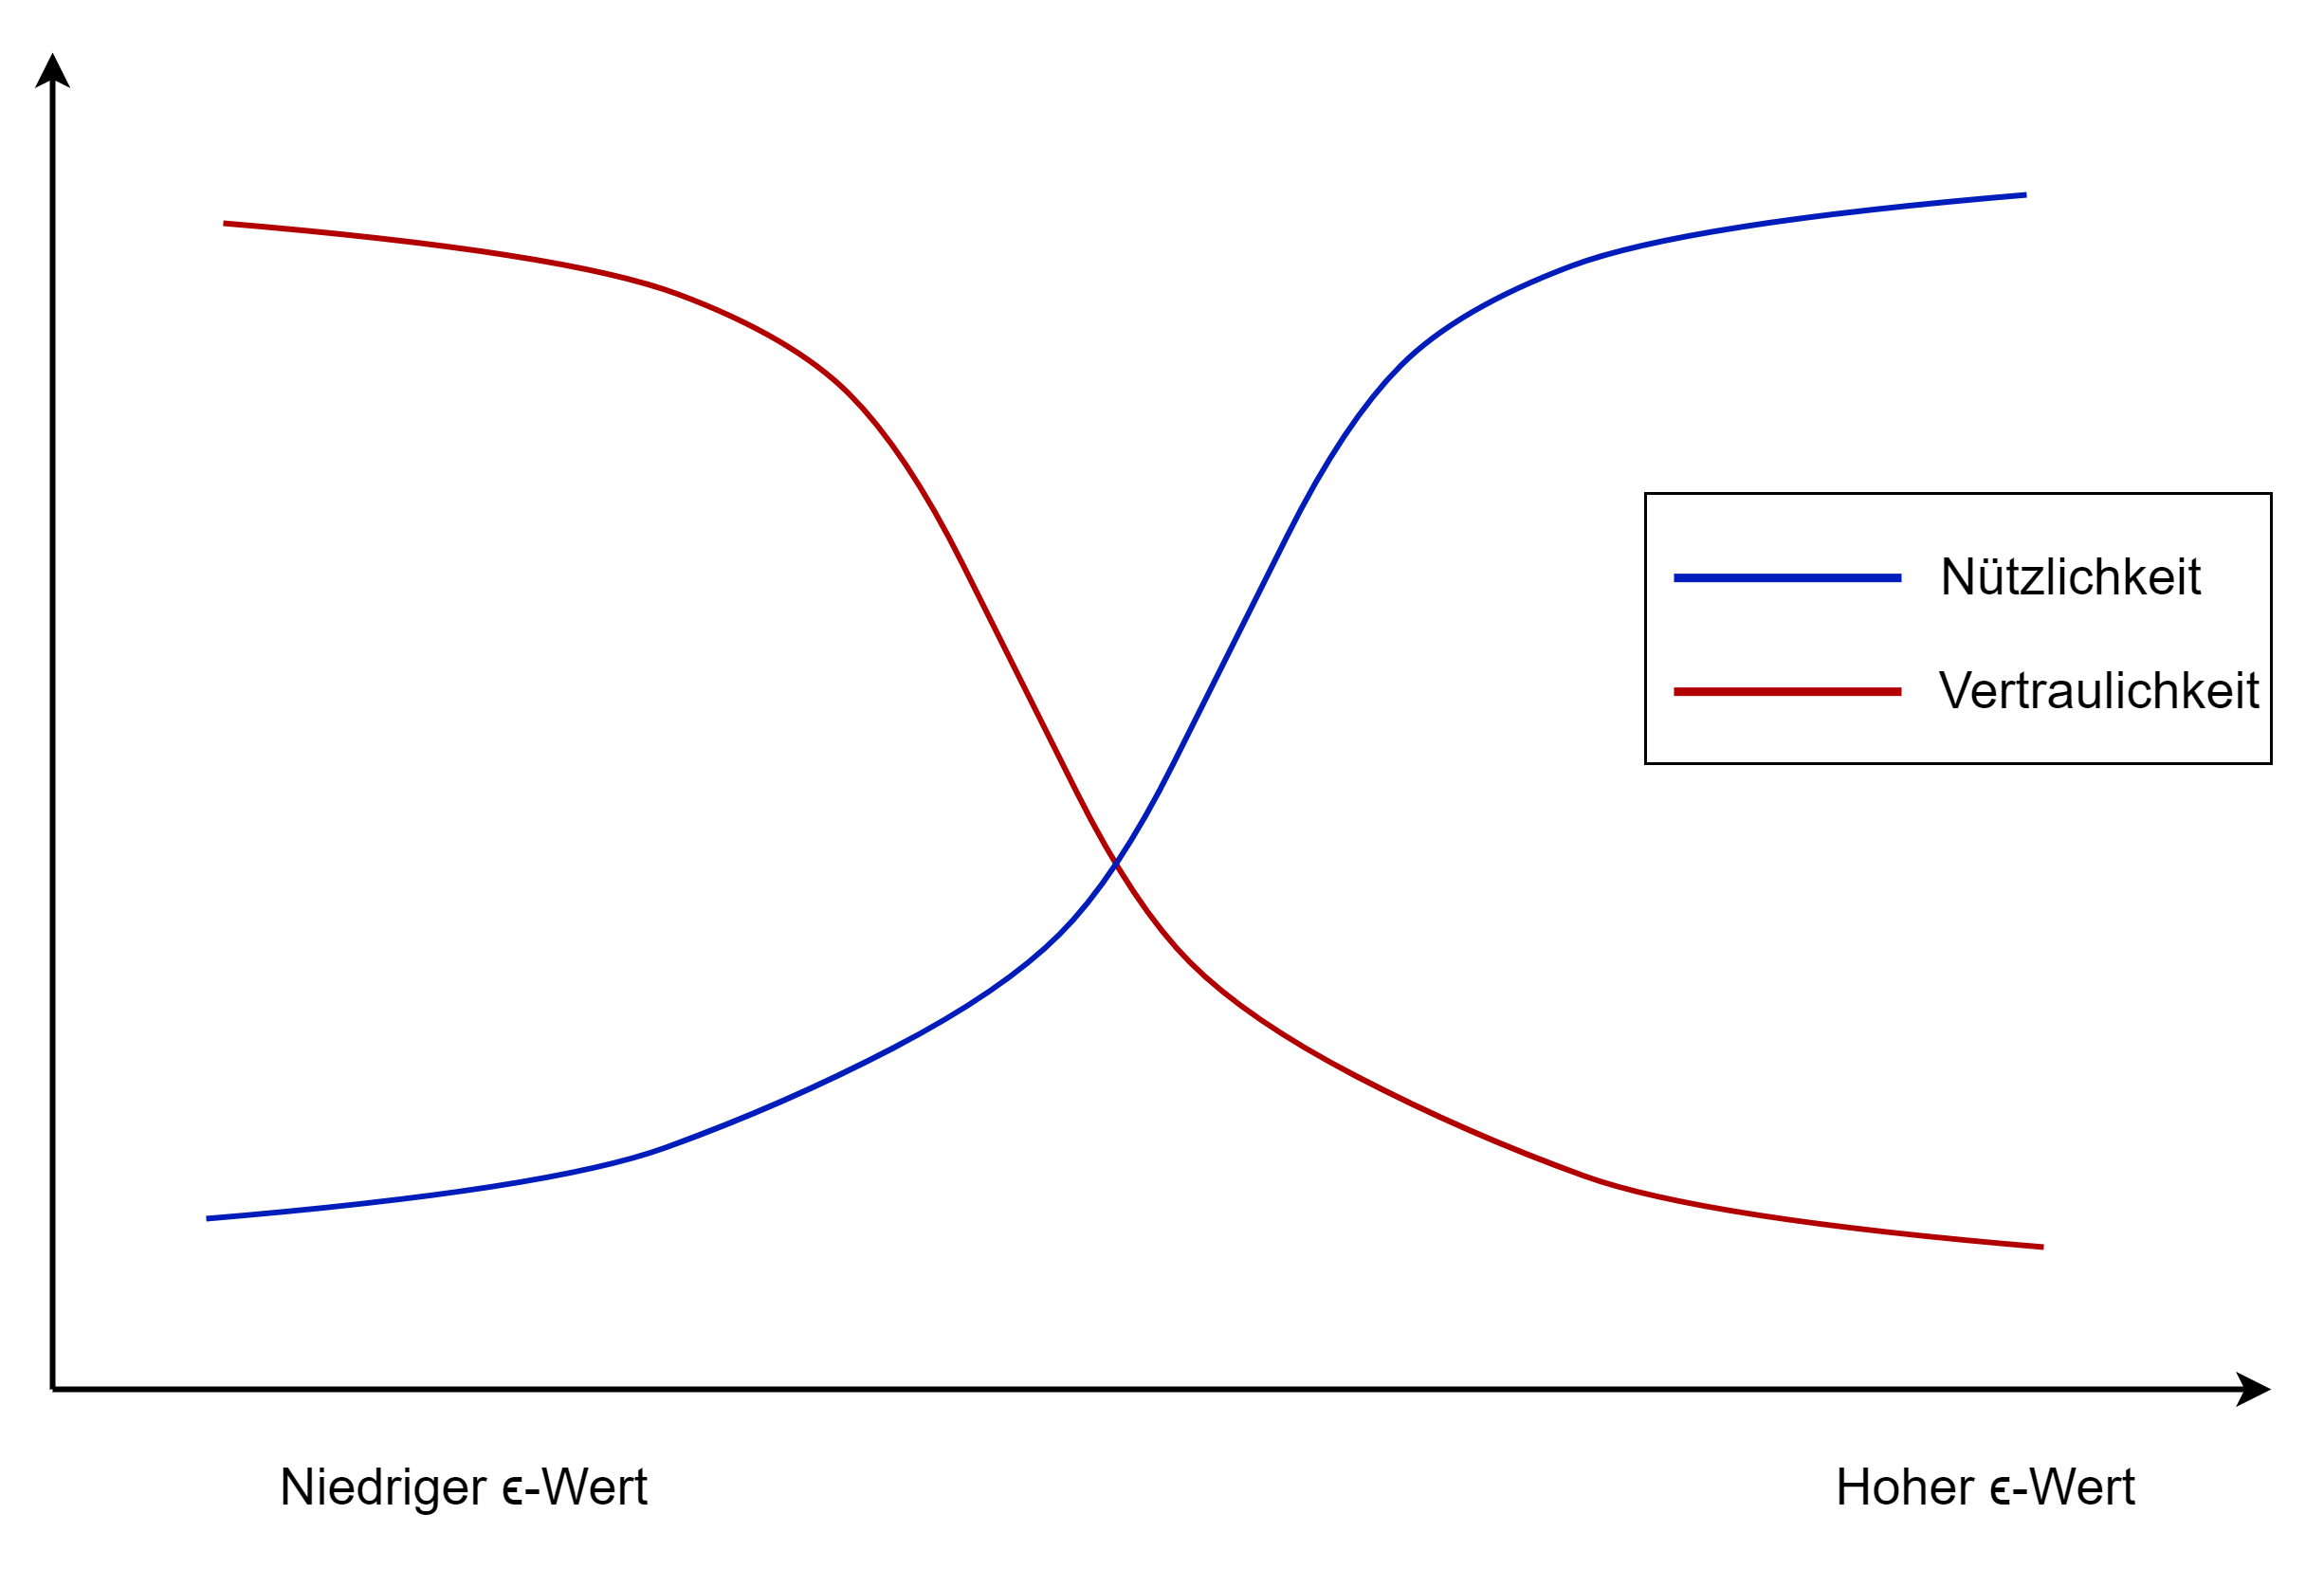
\includegraphics[width=12cm]{figures/dp_privacy_budget.png}
    \caption{Einfluss von $\epsilon$}
    \label{fig:dp_privacy_budget}
\end{figure} 

\subsubsection*{Beispiel für Differential Privacy}

Abbildung \ref{fig:dp} zeigt, wie sich Abfragen mit und ohne Differential Privacy unterscheiden.
Dabei führt ein Angreifer zunächst eine Abfrage über das Durchschnittsgehalt eines Unternehmens auf einem Datenbestand ohne Differential Privacy aus. 
Er erhält hier einen konkreten Wert als Ergebnis.
Anschließend wird der Datenbestand um einen Eintrag erweitert, weil das Unternehmen einen neuen Mitarbeiter hat.
Führt der Angreifer die Abfrage um das Durchschnittsgehalt erneut aus, erhält dieser einen angepassten, neuen Wert.
Dadurch kann er anhand der Anzahl der Mitarbeiter des Unternehmens und der Differenz der beiden Abfragen das exakte Gehalt des neuen Mitarbeiters bestimmen.
Anders sieht dies mit Differential Privacy aus. 
Dabei werden beide Abfragen mit zufälligem Rauschen angereichert. 
Es wird also nur eine Stichprobe einer Verteilung zurückgegeben. 
Bei einer gleichen Abfrage auf den gleichen Datenbestand, können also ebenfalls unterschiedliche Werte zurückgegeben werden.
Führt der Angreifer zwei Abfragen aus, einmal auf dem alten Datenbestand und auf dem Datenbestand mit dem neuen Mitarbeiter, kann er keinen exakten Wert des Gehalts des neuen Mitarbeiters ermitteln.
Differential Privacy bietet einige Algorithmen, wie dieses Rauschen hinzugefügt werden kann, wobei Parameter $\epsilon$ und $\delta$ die Stärke des Rauschens bestimmen und damit auch, wie nah die beiden Ergebnisse aneinander sind.

\begin{figure}[!htb]
    \centering
    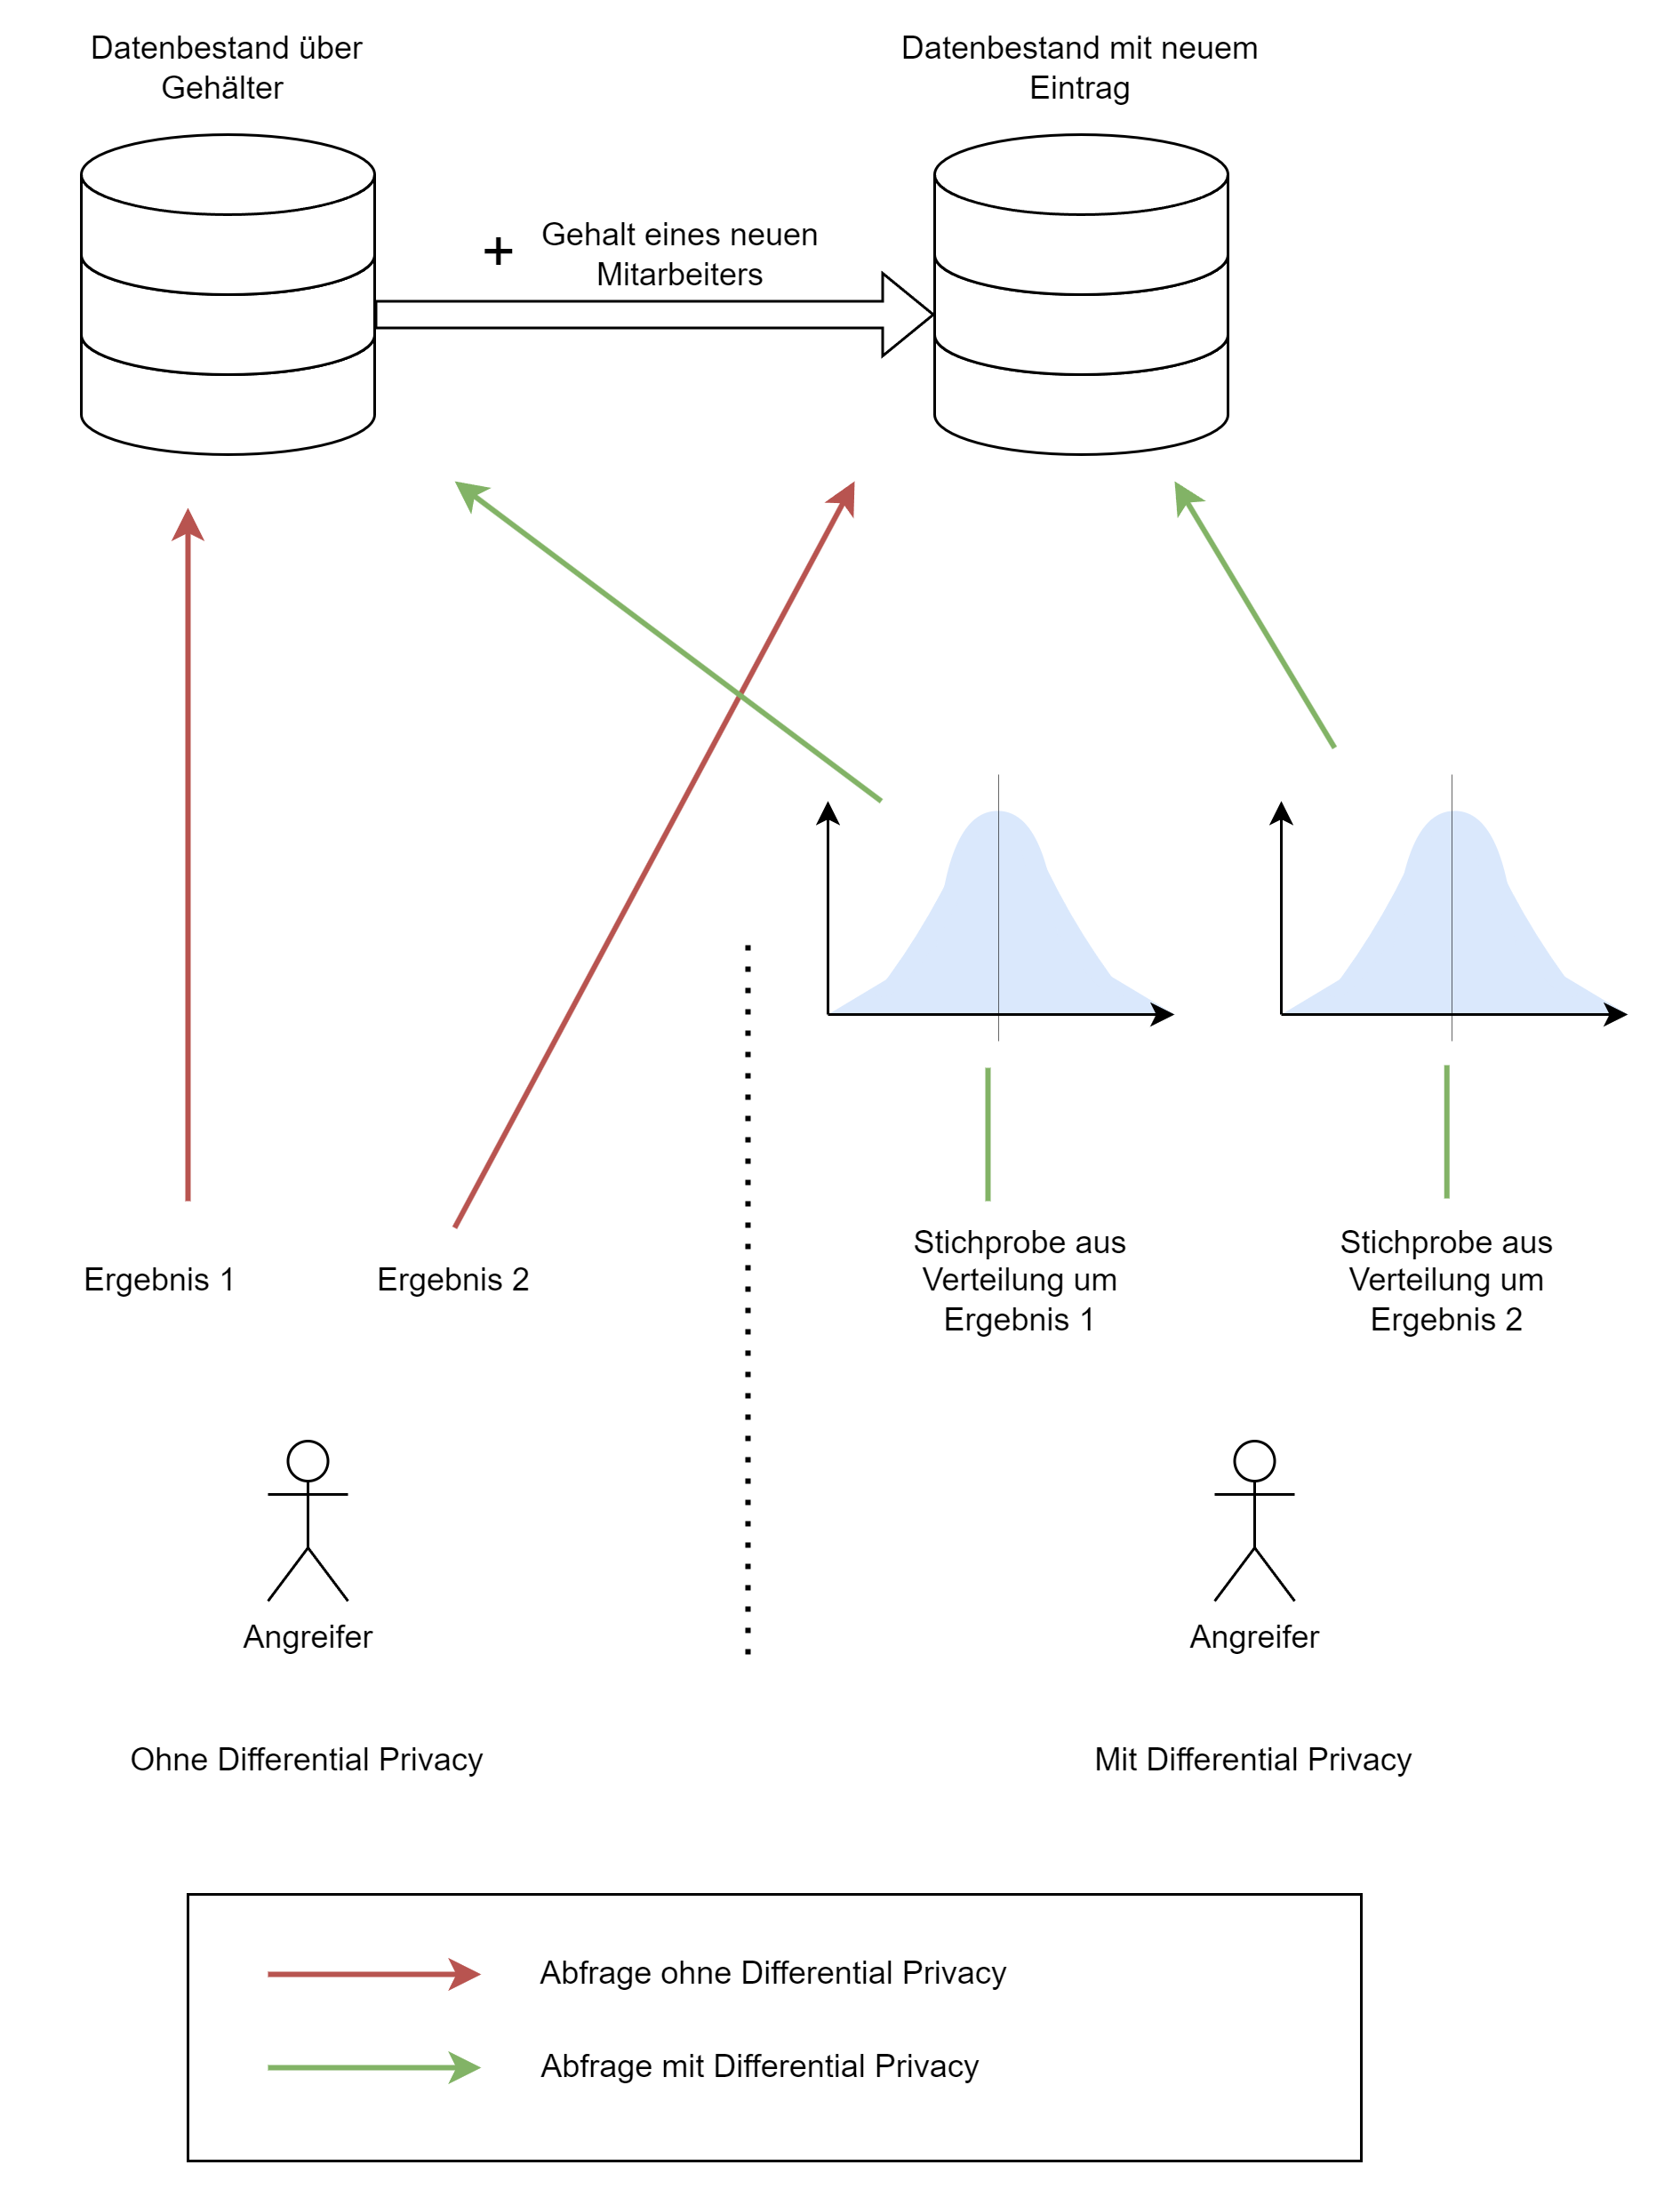
\includegraphics[width=\textwidth]{figures/dp}
    \caption{Beispiel Differential Privacy}
    \label{fig:dp}
\end{figure} 

\subsubsection*{Algorithmen für Differential Privacy}
Die Art des Rauschens, welche über die Ausgabe einer Abfrage gelegt wird, kann unterschiedlichster Herkunft sein.
Dwork und Roth \cite{P-27} stellen eine ganze Reihe dieser Mechanismen vor, die im Folgenden beschrieben werden.

Bei der Technik der randomisierten Antwort, im Englischen Random Response, wird mit einer festgelegten Wahrscheinlichkeit, ein falsches Ergebnis ausgegeben. 
Dies entspricht dem Rauschen dieser Methode.
Wird beispielsweise eine Person gefragt, ob sie eine gewisse Aktivität durchgeführt hat, wird mit 25-prozentiger Wahrscheinlichkeit die falsche Antwort selektiert.
Ist die Wahrheit \textit{\dq Ja\dq}, dann gilt $P[Antwort = \dq Ja\dq \mid Wahrheit = \dq Ja\dq] = 3/4$ und $P[Antwort = \dq Nein\dq \mid Wahrheit = \dq Ja\dq]$.
Gleiches gilt, wenn die Wahrheit \textit{\dq Nein\dq} wäre.
Die jeweils ausgegebene Antwort kann dadurch glaubhaft abgestritten werden.
\begin{equation} \label{formula:random_response}
\begin{split}
\frac{P[Antwort = \dq Ja\dq \mid Wahrheit = \dq Ja\dq]}{P[Antwort = \dq Ja\dq \mid Wahrheit = \dq Nein\dq]} = \frac{3/4}{1/4} = \\
\frac{P[Antwort = \dq Nein\dq \mid Wahrheit = \dq Nein\dq]}{P[Antwort = \dq Nein\dq \mid Wahrheit = \dq Ja\dq]} =  3
\end{split}
\end{equation}

Formel \ref{formula:random_response} zeigt, dass eine Antwort, egal ob diese \textit{\dq Ja\dq} oder \textit{\dq Nein\dq} lautet, mit einem Verhältnis von 3 abgestritten werden kann.
Der Faktor, um den sich die Wahrscheinlichkeit einer Antwort unterscheidet, wenn sich die Wahrheit ändert, liegt demnach auch bei 3.
Daraus resultiert, dass die Technik der randomisierten Antwort, mit einer 25-prozentigen Wahrscheinlichkeit einer falschen Antwort, eine ($ln 3$, 0)-Differential Privacy unterstützt.
Der natürliche Logarithmus $ln$ muss hier genutzt werden, da die Definition von Differential Privacy die Exponentialfunktion als Faktor betrachtet. 
Demnach erhält man durch $\epsilon = ln 3$ einen Unterschied um den Faktor $e^{ln 3} = 3$.

Eine weitere Technik für Differential Privacy ist der Laplace-Mechanismus.
Dabei wird das Rauschen, welches über das Ergebnis der Abfrage gelegt wird, aus einer Laplace-Verteilung ermittelt.
Eine Bedingung ist dabei, dass es sich bei dem Ergebnis der Abfrage um einen Zahlenwert handelt.
Die Dichtefunktion der Laplace-Verteilung, zentriert um den Erwartungswert $\mu=0$, mit dem Skalenparameter $\sigma$, lautet \cite{P-27}:
\begin{equation}
\resizebox{!}{0.55cm}{$
    Lap(x|\sigma) = \frac{1}{2\sigma}\times e^{(-\frac{|x|}{\sigma})}
$}
\end{equation}
wobei $\sigma$ die Steigung der Funktion beeinflusst.
Um nun ein geeignetes $\sigma$ zu wählen, muss zuerst ein Wert ermittelt werden, um den sich eine Funktion bei Änderung eines Datenpunktes maximal unterscheiden kann.
Diese sogenannte Sensitivität wird als $\Delta f$ notiert.
Geht es beispielsweise um eine Anzahl an Datensätzen, so würde ein neuer Datensatz die Anzahl um den Wert 1 erhöhen.
Folglich ist $\Delta f = 1$, denn die Anzahl wird sich durch einen neuen Datensatz um den Wert 1 verändern.
Es gibt jedoch auch Fälle, in denen der Wert der Sensitivität nicht eindeutig ist, beispielsweise bei dem obigen Gehaltsbeispiel.
Das Gehalt einer neuen Person könnte für eine beliebige Veränderung des Durchschnittsgehalts sorgen, da theoretisch jedes Gehalt möglich wäre.
Realistisch betrachtet gibt es jedoch einen Wertebereich, in dem sich alle Gehälter befinden. 
Dieser könnte beispielsweise von 0 Euro bis 10 Milliarden Euro reichen. 
Jedoch sollten die Grenzen möglichst nahe an den echten Grenzen liegen. 
10 Milliarden Euro ist theoretisch möglich, jedoch ist eine Grenze von 200.000 Euro realistischer.
Dieser Wertebereich muss also fachlich festgelegt werden.
In diesem Beispiel wäre die Sensitivität $200.000/n$, wobei $n$ die Anzahl der Mitarbeiter ist.


Um ($\epsilon$,0)-Differential Privacy zu erreichen, muss die Ausgabe einer Abfrage $M$ mit zufälligen Werte der Laplace-Verteilung $Lap(x | \Delta f/\epsilon)$ verrauscht werden \cite{P-27}: 
\begin{equation}
    M(D) = f(D) + (Y_1, ... Y_k),\text{ mit } Y_i \sim Lap(x| \Delta f/\epsilon)
\end{equation}


Eine Abwandlung des Laplace-Mechanismus ist es, anstatt der Laplace-Verteilung, eine Gaußverteilung zu nutzen. Die Dichtefunktion dieser zentriert um den Erwartungswert $\mu=0$ lautet \cite{P-27}:
\begin{equation}\label{formula:gauß}
\resizebox{!}{0.55cm}{$
    Gau\text{\textit{ß}}(x|\sigma) = \frac{1}{\sigma\sqrt{2\pi}}\times e^{-\frac{1}{2}(\frac{x}{\sigma})^2}
$}
\end{equation}
Der Gauß-Mechanismus liefert ($\epsilon$,$\delta$)-Differential Privacy, wenn $\sigma = \Delta f \frac{\text{ln}(1/\delta)}{\epsilon}$ ist \cite{P-27}.

Neben den bereits beschriebenen Mechanismen gibt es noch den Exponential-Mechanismus. 
Bei diesem wird ein Element aus einer Menge ausgegeben, welches anhand einer Bewertungsfunktion ausgewählt wird.
Die Abfrage an einen Datenbestand liefert also keine Zahl, sondern einen Datensatz oder Attributwert aus diesem.
Der Exponential-Mechanismus benötigt eine Bewertungsfunktion $u:D x R \xrightarrow{} \mathbb{R}$, welche für jede potenzielle Ausgabeoption $R$ aus einer Menge an Datensätzen $D$, einen Nutzwert im Wertebereich $\mathbb{R}$ berechnet.
Als Sensitivität $\Delta f$ entspricht der Sensitivität der Bewertungsfunktion $\Delta f = \Delta u$
Die Anfrage erfüllt dabei ($\epsilon$,0)-Differential Privacy, wenn der Mechanismus $M(D,u,R)$ ein Element $r \in R$ auswählt und ausgibt, mit einer Wahrscheinlichkeit proportional abhängig von
\begin{equation}\label{formula:exp_mech}
\resizebox{!}{0.8cm}{$
    e^{\frac{\epsilon \times u(D,r)}{2\Delta u}}
$}
\end{equation}


Als Beispiel könnte ein Mechanismus genutzt werden, welcher ausgeben soll, ob Krankheit \dq A\dq\ oder \dq B\dq\ häufiger vorkommt.
Somit wären die möglichen Optionen $R$=\{\dq A\dq,\dq B\dq\}, die Bewertungsfunktion $u(D,r)=\text{Count(r in D)}$.
Die Sensitivität ist $\Delta u = 1$, da ein zusätzlicher Datensatz die Zählung maximal um die Anzahl 1 verändern kann. 
Für jede der Optionen in $R$, würde die Ausgabewahrscheinlichkeit mit Formel \ref{formula:exp_mech} berechnet werden. 
Anschließend gibt der Mechanismus entweder \dq A\dq\ oder \dq B\dq\ zurück, abhängig der zuvor berechneten Ausgabewahrscheinlichkeiten.
Das Rauschen des Exponential-Mechanismus ist demnach, dass nicht immer die Option $r \in R$ mit dem größten Nutzwert ausgegeben wird. 

Eine alternative Möglichkeit, neben dem Exponential-Mechanismus, einen Wert aus einem Datensatz mittels Ausgabewahrscheinlichkeiten zu bestimmen, ist die sogenannte Report Noisy Max Methode. 
Dabei werden die echten Wahrscheinlichkeitswerte mittels Laplace-Mechanismus verrauscht und anschließend wird der Wert oder Datenpunkt mit der höchsten Wahrscheinlichkeit selektiert.


\subsubsection*{Eigenschaften von Differential Privacy}
Das Ziel von Differential Privacy, die Vertraulichkeit eines Datensatzes zu schützen und dennoch die Nützlichkeit des Datenbestands zu bewahren, wurde bereits zu Beginn des Kapitels geschildert.
Jedoch bringt Differential Privacy eine Reihe weiterer nützlicher Eigenschaften mit sich \cite{P-27}:
\begin{compactitem}
    \item \textbf{Gruppen Privacy:} Differential Privacy betrachtet zwei Datenbestände, die sich in einem Datensatz unterscheiden. Jedoch gelten die gleichen Regeln für Datenbestände, die sich in mehreren Datensätzen unterscheiden, wobei $\epsilon$ dabei mit der Anzahl der unterschiedlichen Datensätze multipliziert wird.
    \item \textbf{Resistenz gegen Umkehrung bei der Weiterverarbeitung:} Das Ergebnis eines Mechanismus, welcher Differential Privacy nutzt, ist geschützt und es gibt keinen Mechanismus, welcher dies umkehren könnte. Somit sind geschützte Weiterverarbeitungen der Ergebnisse möglich.
    \item \textbf{Quantifizierung der Vertraulichkeit:} Mit den Parametern $\epsilon$ und $\delta$ kann angegeben werden, wie stark die Vertraulichkeit der Daten geschützt wird.
    \item \textbf{Bewertung zusammengesetzter Mechanismen:} Durch die Quantifizierung der Vertraulichkeit, können auch zusammengesetzte und parallele Berechnungen bewertet werden.
\end{compactitem}



Die Bewertung von mehreren zusammengesetzten Mechanismen ist dabei komplex und kann für bestimmte Berechnungen verfeinert werden \cite{P-27}. 
Der dabei berechnete $\epsilon$-Wert ist eine Obergrenze, welcher durch bestimmte Restriktionen und Berechnungen noch genauer definiert werden kann.
Grundlegend jedoch, besitzt ein Mechanismus, welcher aus nacheinander ausgeführten Teilmechanismen besteht, einen $\epsilon$-Wert und $\delta$-Wert, welcher der Summe aus den einzelnen Teilmechanismen entspricht.
Erfüllt $M_1(D)$ eine $(\epsilon_1,\delta_1)$-Differential Privacy und $M_2(D)$ eine $(\epsilon_2,\delta_2)$-Differential Privacy, dann erfüllt der gesamte Mechanismus $(\epsilon_1 + \epsilon_2,\delta_1 + \delta_2)$-Differential Privacy.
Wird ein und derselbe Teilmechanismus mit $(\epsilon,\delta)$-Differential Privacy $t$ mal ausgeführt, so entspricht der Gesamtmechanismus $(t\epsilon,t\delta)$-Differential Privacy.
Zusammengefasst lässt sich dies durch folgende Definition beschreiben \cite{P-27}:\\
\textit{
    Wenn ein Mechanismus $M_{|t|}$, aus $t$ Teilmechanismen $M_i$ mit $(\epsilon_i,\delta_i)$-Differential Privacy besteht, dann erfüllt dieser  ($\Sigma_{i=1}^{t} \epsilon_i $, $\Sigma_{i=1}^{t} \delta_i $)-Differential Privacy
}

Alternativ kann ein Mechanismus auch aus Teilmechanismen bestehen, welche jeweils nur auf einer disjunkten Menge an Datensätzen des gesamten Datenbestands ausgeführt wird.
Der gesamte Mechanismus hat als $\epsilon$ und $\delta$-Wert dabei die maximalen Werte der Teilmechanismen.\\
\textit{
    Wenn ein Mechanismus $M_{|t|}$, aus $t$ Teilmechanismen $M_i$ mit $(\epsilon_i,\delta_i)$-Differential Privacy besteht, welche jeweils 
    nur auf einer disjunkten Menge an Datensätzes des gesamten Datenbestands $D_i$ ausgeführt werden, 
    dann erfüllt dieser Mechanismus ($max_i(\epsilon_{i})$, $max_i(\delta_{i})$)-Differential Privacy
}


Ein Beispiel für einen Algorithmus, welcher eine angepasste Bewertung von zusammengesetzten Mechanismen besitzt, ist der Trainingsalgorithmus DPSGD (Kapitel \ref{sec:dp_training}) \cite{P-28}.
Diese Anpassung sorgt dafür, dass der $\epsilon$-Wert über den ganzen Trainingsprozess möglichst niedrig bleibt.
Ziel davon ist es, eine Obergrenze für $\epsilon$ zu beschreiben, welche näher an den tatsächlichen Berechnungen liegt, als das Aufsummieren der einzelnen $\epsilon$ Werte.


\subsubsection*{Vorverarbeitung der Trainingsdaten}
Um die Trainingsdaten eines Modells mit Differential Privacy zu schützen, ist es möglich, die Daten vor der Eingabe in das Modell zu verrauschen.
Der Forward-Pass eines Modells wird demnach nicht auf den echten Daten ausgeführt, sondern auf den jeweils verrauschten Versionen der einzelnen Datensätze.

Um einen einzelnen Datensatz zu verrauschen, muss jedes Attribut des Datensatzes individuell betrachtet werden. 
Dabei ist die Sensitivität individuell zu setzen, beeinflusst von statistischen Merkmalen des Attributes.
Ebenfalls kann sich der Differential Privacy Mechanismus unterscheiden, abhängig davon, ob es sich um kategoriale oder numerische Werten handelt.
Bei numerischen Werten kann der Laplace-Mechanismus oder Gauß-Mechanismus gewählt werden, bei kategorialen Werten der Exponential-Mechanismus.
Der $\epsilon$-Wert und $\delta$-Wert eines einzelnen Datenpunktes entspricht anschließend der Summe der Werte des einzelnen Verrauschens jeder Variable.

Da jeder Datensatz alleine eine disjunkter Menge des Datenbestands darstellt, gilt, dass der $\epsilon$-Wert und $\delta$-Wert dem Maximum des Rauschens auf die einzelnen Datensätze entspricht.
Wird also jeder Datensatz mit dem gleichen, festgelegten Mechanismus mit ($\epsilon$,$\delta$)-Differential Privacy verrauscht, dann entspricht dies auch den Werten des gesamten Vorverarbeitungsprozess.

Alternativ kann ein ganzer Datenbestand mit Differential Privacy geschützt werden, indem dieser nur dazu genutzt wird, einen synthetischen Datenbestand zu erzeugen.
Dieser kann anschließend wie der originale Datenbestand genutzt werden.
Das folgende Kapitel stellt einige Methoden dazu vor.


\subsection{Synthetische Daten}\label{sec:synthetic_data}

Bei einem synthetischen Datenbestand handelt es sich um einen künstlich erzeugten Datenbestand, welcher die gleichen statistischen Merkmale wie der ursprüngliche Datenbestand enthält.
Statistische Abfragen oder auch komplexere Modelle, wie neuronale Netze, sollen demnach bei beiden Datenbeständen vergleichbare Ergebnisse liefern.

Bisher wurde Differential Privacy für einzelne Abfragen genutzt.
Es gibt jedoch auch Verfahren, welche es ermöglichen, eine synthetische Menge an Datensätzen zu veröffentlichen, welcher mit Differential Privacy geschützt werden.
Hardt \etal \cite{P-90} stellen solch ein Verfahren vor, welches MWEM genannt wird.
Dieses basiert auf Marginalverteilungen, auch Randverteilungen genannt, von verschiedenen Attributen zueinander.
Dabei handelt es sich um Anzahlen verschiedener Attributwerte eines Attributs in Kombination mit den Anzahlen verschiedener Attributwerte eines anderen Attributes.
Einzelne Werte der Marginalverteilungen werden auch Marginalhäufigkeiten genannt.
Tabelle \ref{tab:marginals} zeigt, wie ein Beispiel von Marginalverteilungen zwischen den Attributen \dq A\dq\ und \dq B\dq, welche jeweils zwei unterschiedliche Attributwerte annehmen können.
Stetige Werte müssten vorher in verschiedene Klassen gruppiert werden.

% Please add the following required packages to your document preamble:
% \usepackage[table,xcdraw]{xcolor}
% If you use beamer only pass "xcolor=table" option, i.e. \documentclass[xcolor=table]{beamer}
\begin{table}[!htb]
\centering
\begin{tabular}{|
>{\columncolor[HTML]{CBCEFB}}l |l|l|l|}
\hline
                   & \cellcolor[HTML]{CBCEFB}Attributwert \dq $A_{1}$\dq & \cellcolor[HTML]{CBCEFB}Attributwert \dq $A_{2}$\dq & \cellcolor[HTML]{CBCEFB}Marginalverteilung \\ \hline
Attributwert \dq $B_{1}$\dq    & 10                                      & 5                                       & 15                                         \\ \hline
Attributwert \dq $B_{2}$\dq    & 13                                      & 4                                       & 17                                         \\ \hline
Marginalverteilung & 23                                      & 9                                       & 32                                         \\ \hline
\end{tabular}
\caption{Beispiel Marginalverteilungen\cite{D-titanic}}
\label{tab:marginals}
\end{table}

Um eine Datenmenge umzuwandeln, wird eine Datenmenge $D'$ mit der gleichen Anzahl an Elementen wie die ursprüngliche Datenmenge $D$ initialisiert, wobei die Initialwerte der Attribute mittels einer Gleichverteilung über alle potenziellen Attributwerte des jeweiligen Attributes ermittelt werden.
Das Verfahren besteht aus 3 Schritten, welche iterativ wiederholt werden können, um die künstliche Datenmenge $D'$ an die echte Datenmenge $D$ anzugleichen:
\begin{compactenum}
    \item \textbf{Wahl einer Anfrage:} Aus allen Marginalhäufigkeiten der ursprünglichen Datenmenge, wird mittels Exponential-Mechanismus die Marginalhäufigkeit gewählt, die den größten Unterschied zwischen den Eingaben $D'$ und $D$ besitzt.
    Die Bewertungsfunktion $u$ des Exponential-Mechanismus bewertet folglich die Differenzen der Marginalverteilungen der beiden Datenmengen (originale Datenmenge und synthetische Datenmenge).
    \item \textbf{Verrauschen:} Mittels Laplace-Mechanismus wird nun das Ergebnis der gewählten Marginalverteilung aus Schritt 1 verrauscht.
    \item \textbf{Anpassen von $D'$:} Abhängig von dem verrauschten Ergebnis der gewählten Marginalverteilung, werden die Attributwerte von $D'$ so angepasst, dass die Marginalverteilungen sich angleichen.
\end{compactenum}
Nach Beendigung des Algorithmus, ist $D'$ eine synthetische Datenmenge, welche die originale Datenmenge $D$ mit Differential Privacy abbildet.

Die Erzeugung synthetischer Daten wurde im Jahre 2016 maßgeblich durch die Generative Adversarial Network Architektur, auch GAN genannt, beeinflusst \cite{P-86}. 
Bei dieser Architektur gibt es zwei gegensätzliche neuronale Netzwerke, der Generator und der Diskriminator. 
Der Diskriminator lernt dabei, zwischen echten Daten und nicht echten Daten zu unterscheiden, welche abwechselnd von dem echten Datenbestand und von dem Generator kommen.
Im Gegensatz dazu, versucht der Generator, Datensätze zu erzeugen, die den Diskriminator täuschen. 
Der Diskriminator kann dabei zwei Verlustfunktionen haben, einmal für sich selber und einmal für den Generator.
Die Verlustfunktion des Generators kann dabei durch den Generator backpropagiert werden, wodurch dieser immer realistischere Datensätze generiert.
Im besten Falle, erzeugt der Generator nach dem Training Datensätze, die so echt wirken, dass der Diskriminator diese nicht mehr unterscheiden kann.
Folglich erzeugt der Generator synthetische Daten, welche die statistischen Strukturen der originalen Daten enthalten.
Abbildung \ref{fig:gan} zeigt die bereits beschriebene Architektur.

\begin{figure}[!htb]
    \centering
    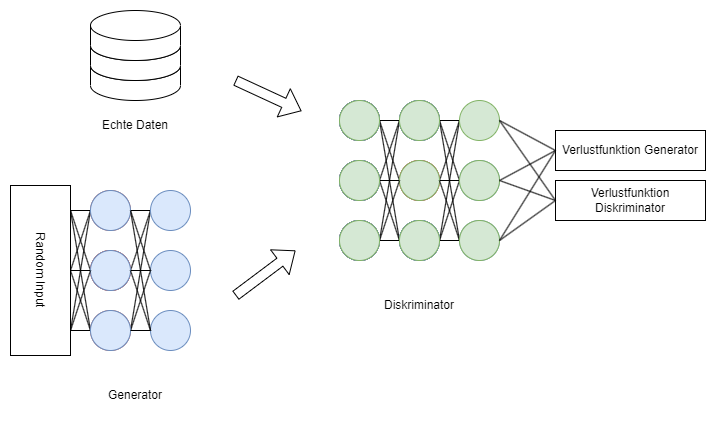
\includegraphics[width=14cm]{figures/gan}
    \caption{Generative Adversarial Network nach \cite{P-86}}
    \label{fig:gan}
\end{figure} 

Die Erzeugung von Daten mittels GANs kann nicht nur für Angriffe genutzt werden (siehe Kapitel \ref{sec:angriffe}), sondern auch für das Training von neuronalen Netzen.
Eine Erweiterung der GANs ist das sogenannte Wasserstein GAN oder auch kurz WGAN \cite{P-92}. 
Standardmäßig kann bei GANs der Fall auftreten, dass die erzeugten Daten nicht jeden Teil einer Verteilung abbilden, sondern nur einen Teil, \zB den am häufigsten vorkommenden Datensatz.
Um dieses Problem zu mindern, wird beim WGAN die Verlustfunktion des Diskriminators verändert. 
Anstatt einer binären Klassifikation (echt oder unecht), wird die Wasserstein-Distanz genutzt, welche angibt, wie viel Arbeit benötigt wird, um eine Verteilung in eine andere Verteilung zu transformieren. 
Die Wasserstein-Distanz gleicht der Earth-Mover-Distanz aus Kapitel \ref{sec:anonymisierung}.
Diese Metrik als Verlustfunktion ist jedoch nur nützlich, wenn nicht mit einzelnen Datensätzen, sondern jeweils mit Batches trainiert wird.
Der Austausch der Verlustfunktion sorgt dafür, dass der Generator Daten aus der ganzen Verteilung der Daten nachstellen muss und nicht nur aus einem Teil dieser.


Xie \etal \cite{P-70} stellen eine besondere Form des GANs vor, das sogenannte Differentially Private Generative Adversarial Network oder kurz DPGAN.
Dieses DPGAN nutzt als Basis das WGAN, fügt jedoch bei Berechnung der Verlustfunktion (Wasserstein-Distanz) Rauschen mittels des Gauß-Mechanismus aus Kapitel \ref{sec:dp} hinzu.
Durch die Eigenschaft, dass Differential Privacy resistent gegenüber Nachbearbeitung ist, kann auch garantiert werden, dass die Gradienten, die im Generator ankommen, mittels Differential Privacy geschützt sind.
Die Autoren können zeigen, dass es möglich ist, Bilder der MNIST Datenmenge \cite{D-MNIST} zu erzeugen.
Abbildung \ref{fig:dpgan} zeigt diese Erzeugung mit unterschiedlichen $\epsilon$ Werten.
Es ist zu sehen, dass bei kleiner werdendem $\epsilon$, die Qualität der Bilder schlechter wird und auch mehr Daten der falschen Klasse erzeugt werden. 
Bei $\epsilon=9,6$ ist die Anzahl an Daten mit falschem Label größer, als die Anzahl der Daten mit richtigem Label.
Folglich ist die Wahl von $\epsilon$ entscheidend, wie gut die synthetischen Daten die Originaldaten wiedergeben.
Die Wahl muss von $\epsilon$ muss dabei für jeden Use Case neu evaluiert werden.

\begin{figure}[!htb]
    \centering
    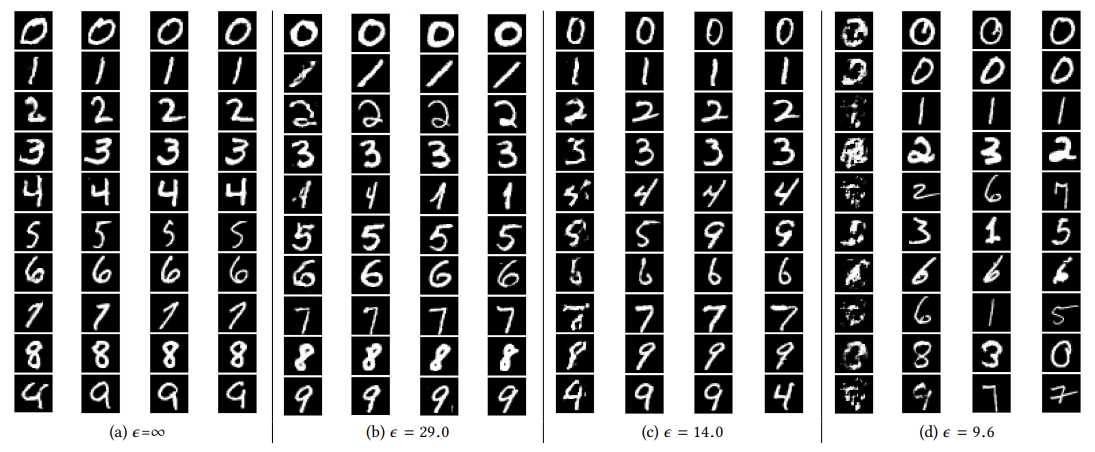
\includegraphics[width=\textwidth]{figures/dpgan}
    \caption{Synthetische MNIST Datenmenge mittels DPGAN \cite{P-70}}
    \label{fig:dpgan}
\end{figure} 

Jordon \etal \cite{P-68} stellten eine alternative Form des GANs vor, welches ebenfalls synthetische Daten erzeugt. 
Dieses nutzt das Private Aggregation of Teacher Ensembles Framework, kurz PATE, welches in Kapitel \ref{sec:pate} im Detail beleuchtet wird.
Bei der PATE-Architektur wird der Datenbestand in verschiedene Teildatenmengen unterteilt. 
Verschiedene Modelle, die sogenannten Lehrer oder Teacher Modelle, lernen die Klassifikation jeweils an einer der unterschiedlichen Teildatenmengen.
Ein weiteres Modell, welches Schüler oder Student Modell genannt wird, kann nun mittels des Exponential-Mechanismus aus \ref{sec:dp} aus den aggregierten Vorhersagen der Lehrer Modelle, eine Klasse vorhersagen.
Das PATE-GAN nutzt die PATE-Architektur für den Diskriminator, welcher ein binärer Klassifikator ist.
Wie das DPGAN, nutzt auch das PATE-GAN die Resistenz gegenüber Nachbearbeitungen von Differential Privacy aus, um Differential Privacy auch für die synthetischen Daten zu garantieren.


Ein weiterer Algorithmus, welcher kein GAN zur Erzeugung künstlicher Daten nutzt, ist NIST-MST von McKenna \etal \cite{P-95}.
Mit NIST-MST gewannen McKenna \etal die \textit{Differential Privacy Synthetic Data Competition}, welche vom National Institute of Standards and Technology der USA ausgetragen wurde.
Neben NIST-MST, welcher auf den obigen Wettbewerb angepasst wurde, gibt es noch MST für generelle Anwendungsfälle.
Die MST Methode basiert, wie MWEM \cite{P-90}, auf Marginalverteilungen.
MST besteht dabei aus 3 Schritten \cite{P-95}:
\begin{compactenum}
    \item \textbf{Wahl von Marginalverteilungen:} Aus dem Datenbestand, über den synthetische Daten erzeugt werden, können mehrere Marginalverteilungen gewählt werden. Dabei sollten die wichtigsten Zusammenhänge und Abhängigkeiten des Datenbestands in diesen vorkommen. Es wird deshalb empfohlen, dass ein Fachexperte die Marginalverteilungen aussucht.
    \item \textbf{Zählen der Marginalverteilungen:} Marginalverteilungen enthalten die Anzahl von Attributwerten eines Attributes in Abhängigkeit von den Attributwerten eines anderen Attributes. Um die Vertraulichkeit der Daten mittels Differential Privacy zu schützen, werden die unterschiedlichen Anzahlen der Variablen mittels Gauß-Mechanismus verrauscht.
    \item \textbf{Erzeugung der Daten:} MST nutzt ein Tool namens Private-PGM \cite{P-97}, welches von den gleichen Autoren stammt, um einen künstlichen Datenbestand zu erzeugen. Dabei sollen die Marginalverteilungen des künstlichen Datenbestands möglichst nahe an den gemessenen Marginalverteilungen liegen.
\end{compactenum}
Die MST Methode ähnelt der MWEM Methode, jedoch gibt es einige Unterschiede.
MWEM ist ein iterativer Algorithmus, welcher in jeder Iteration die Marginalhäufigkeit mit der größten Differenz zwischen originalem Datenbestand $D$ und synthetischem Datenbestand $D'$ wählt und die Attributwerte des synthetischen Datenbestands so anpasst, dass diese sich der Marginalhäufigkeit des originalen Datensatzes angleicht.
MST hingegen stellt mit dem Tool Private-PGM \cite{P-97} ein Optimierungsproblem auf, welches versucht, einen Datenbestand zu finden, dessen Marginalverteilungen möglichst Nahe an den gemessenen Marginalverteilungen des originalen Datenbestands liegt.